% ============================================================================================
% PAPER 1, SHORT FORMAT (PRL): skeleton + first-draft text. Started 2026-10-14.
% Scope (user, 2026-10-13): cavities only; the channel appears once, as the flat limit of the wall law.
% Length target: PRL 3750 words incl. captions (~4 figures). Current draft: see `texcount` (TODO).
% Numbers come from reports/theory_report (26 pp, 2026-10-14) and RESEARCH.md. Every
% "TODO" marks a decision or a missing piece; "%%" comments give the figure plan.
% Figures: placeholders reuse the report's vector PDFs; the final figures are composites (see plan).
% ============================================================================================
\documentclass[aps,prl,twocolumn,superscriptaddress,amsmath,amssymb,reprint]{revtex4-2}
\usepackage{graphicx}
\usepackage{xcolor}
\usepackage[hidelinks]{hyperref}
\graphicspath{{figs/}{../../theory_report/figs/}}
\DeclareGraphicsExtensions{.pdf,.png}
\newcommand{\half}{\tfrac12}
\newcommand{\la}{\ell_a}
\newcommand{\kT}{k_BT}
\newcommand{\todo}[1]{\textcolor{red}{[TODO: #1]}}

\begin{document}

\title{Flow alignment sets the topological charge of active nematic cavities}
%% Alternatives: "Why an active nematic cavity holds one charge in its bulk"; "Topological overcharging of active nematics by confined flow"
\author{Benjamin Loewe}
\affiliation{Facultad de F\'isica, Pontificia Universidad Cat\'olica de Chile, Santiago 7820436, Chile}
\author{Tyler N. Shendruk}
\affiliation{School of Physics and Astronomy, The University of Edinburgh, Peter Guthrie Tait Road, Edinburgh EH9 3FD, United Kingdom}
\date{\today}

\begin{abstract}
A cavity whose wall anchoring winds $k$ times must hold topological charge $k$. A passive nematic places all $2k$ half-integer defects at the wall. An active
nematic keeps exactly $2k-2$ at the wall and moves a net charge $+1$ into the bulk. Using particle-based simulations and continuum theory, we show that this
overcharging is set by flow, not elasticity. The anchoring selects $2k-2$ wall sites and ties each wall defect's tilt to its position, so a common tilt imposed by
the active vortex is a free deformation of a ring of $2k-2$ but frustrates a ring of $2k$, which ejects two defects. The tilt is the flow-aligned angle in the
no-slip shear at the wall, $\arccos(1/\lambda)$, which we confirm across the flow-alignment parameter $\lambda$. The same tilt turns each wall defect's active jet
along the wall and protects the layer; in elongated cavities the coherent vortex is lost, the jets turn inward and the layer leaks, until the bulk holds a fixed
charge per unit wall length set by the winding density.
\end{abstract}
\maketitle

% --------------------------------------------------------------------------------------------
%% INTRODUCTION (~4 paragraphs). TODO(Benjamin): framing and literature; below is a placeholder argument.
Confining an active nematic turns its chaotic flows into coherent ones: circulating vortices in disks, laminar or dancing states in channels
\cite{Doostmohammadi2018,Theillard2017,Opathalage2019,Shendruk2017,Hardouin2019}, and active boundary layers at the walls \cite{Hardouin2022}. Anchoring at the walls also fixes the total topological charge, and patterned anchoring lets one impose any winding $k$.
A passive nematic satisfies this constraint at the wall. An active nematic, as we show, does not: in a circular cavity of winding $k$ it keeps
$2k-2$ defects of charge $+\half$ at the wall and sends a net $+1$ into the bulk, for every $k$ we tested and at every size above about one active length.
Norton \emph{et al.}\ imposed boundary charges $-1$, 0 and $+1$ on continuum active nematics in disks and found the dynamics insensitive to topology: in the
turbulent state the boundary charge is held in a thin topological boundary layer around a neutral interior \cite{Norton2018}. Klein \emph{et al.}\ imposed larger
windings, with up to ten excess $+\half$ defects, below the turbulence threshold, where the defects braid in periodic orbits and tend to screen the excess
charge at the boundary \cite{Klein2026}. Here we impose windings up to $k=10$ in the turbulent regime, with continual pair creation, and find that the boundary
does not screen the excess charge completely: exactly $+1$ always enters the bulk, and in non-circular cavities far more. Topology is screened, geometry is not.
\todo{check the wording of the novelty claim against \cite{Norton2018,Klein2026}; citation search ("cited by") still to do}

Here we identify the mechanism. \todo{one paragraph summarising the three results: (i) symmetry + lock + flow-induced ejection; (ii) tilt law; (iii) elongation, escape, wall law}

% --------------------------------------------------------------------------------------------
\paragraph*{Model.} We simulate a two-dimensional active nematic with multi-particle collision dynamics (MPCD, NIAMH-MPCD \cite{Kozhukhov2022}): extensile active
dipoles, activity $\zeta=0.07$ (active length $\la=22.2$ cells \cite{Kozhukhov2024}), measured Frank constants $K_1\approx42\,\kT$ (splay) and $K_3\approx23\,\kT$ (bend), and flow-alignment
parameter $\lambda=2$ unless stated. No-slip walls impose strong anchoring with director angle $\theta=k\phi$ along the wall (uniform in arclength for non-circular walls).
Cavities are circles of radius $R=0.3$--$2.9\,\la$ with $k=2$--10, and ellipses and Cassini ovals of aspect ratio 1.1--2.5 at three sizes (675 runs). Details in the SM.

% --------------------------------------------------------------------------------------------
%% FIG. 1 (composite, full width): (a) passive vs active density maps (maps_circles a, d-f); (b) anchoring sketch with 2k-2 homeotropic points and the lock (fig_lock);
%% (c) wall count and bulk charge vs R/l_a for k = 2..10 (TODO: new panel from the circle sweep, server seeds); (d) snapshot with tilted wall defects and the vortex (TODO).
\begin{figure}[t]
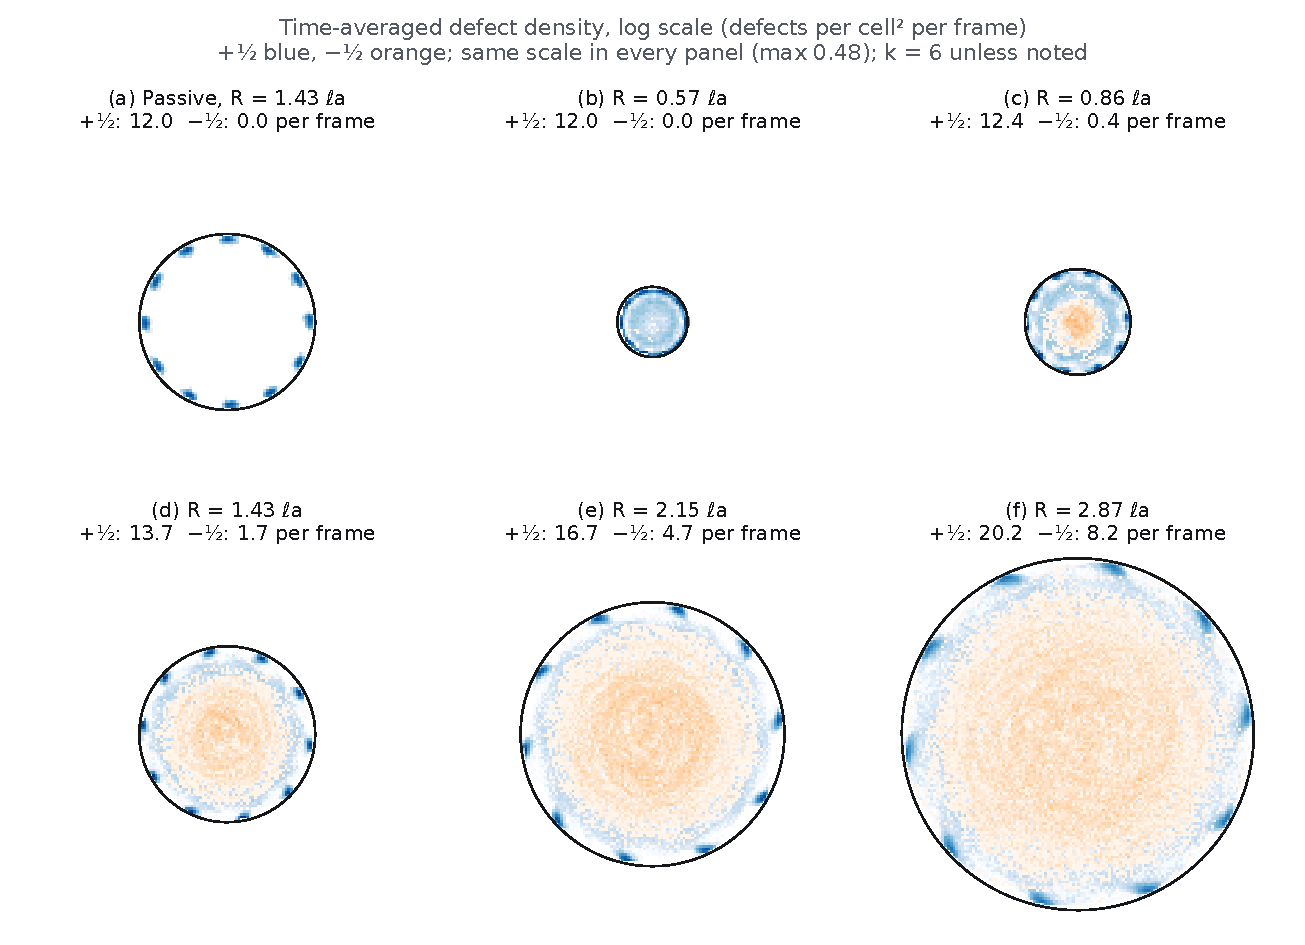
\includegraphics[width=\columnwidth]{maps_circles}
\caption{\todo{composite Fig.~1, see plan in the source}. Time-averaged defect density in circular cavities with $k=6$: passive (12 $+\half$ at the wall) and active
at increasing $R/\la$ (10 wall sites and a bulk $+1$ above $R\approx0.8\,\la$).}\label{fig:obs}
\end{figure}

\paragraph*{Observation.} In passive cavities all $2k$ $+\half$ defects sit in a ring at the wall (Fig.~\ref{fig:obs}). With activity, and for $R\gtrsim0.8\,\la$, the wall
holds exactly $2k-2$ sharply localised defects and the bulk a net charge $+1$, while $\pm\half$ pairs are created and annihilated in the bulk. A single vortex fills
the cavity, and the wall defects are tilted by $\approx62^\circ$ from the wall normal, all in the sense of the vortex. \todo{state the k and size range, seeds, and the
fraction of time in the overcharged state from the server production runs}

\paragraph*{Anchoring geometry.} Relative to the local wall normal the anchored director turns by $(k-1)\phi$, so it is homeotropic at $2k-2$ points
$\phi_n=2\pi n/(2k-2)$. A wall $+\half$ at azimuth $\phi_j$ has its tail tilted from the normal by
\begin{equation}
\tau_j=(2k-2)\phi_j+\text{const},\label{eq:lock}
\end{equation}
which the simulations obey with a mean resultant length 0.99. Tilt and position are one degree of freedom: a common tilt of a ring is a rigid shift of its registry.
A ring of $2k-2$ defects can therefore sit untilted on the homeotropic points, and tilt as a whole at no elastic cost. A ring of $N=2k$ evenly spaced defects cannot:
by Eq.~\eqref{eq:lock} consecutive tilts differ by $-2\pi/k$ and wind twice around the ring. With unequal splay and bend constants the commensurate ring is pinned
to the sites (barrier 80--110\,$\kT$ at $k=6$), and the incommensurate one is not.

% --------------------------------------------------------------------------------------------
%% FIG. 2 (mechanism): (a) energy of the ejected structure vs the 2k ring under a common tilt (tilted_structures b); (b) passive cavity + imposed vortex: wall count and
%% tilt coherence vs time (fig_ejection); (c) continuum active Q-tensor with backflow: same state (TODO: snapshot panel from shear_tilt/active_bf).
\begin{figure}[t]
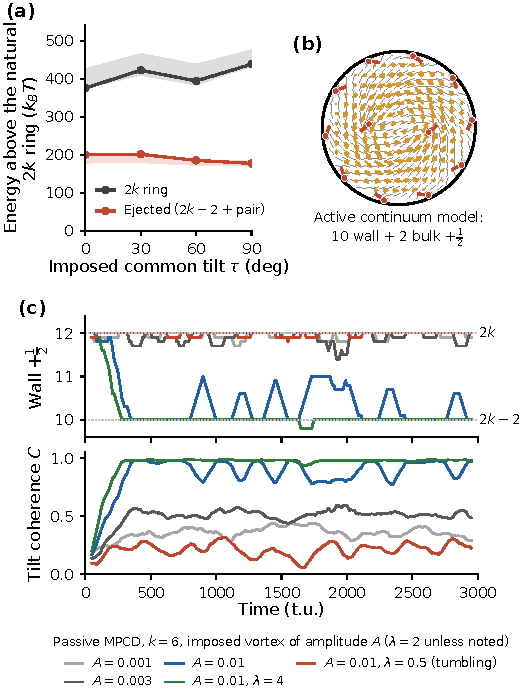
\includegraphics[width=\columnwidth]{fig2_mechanism}
\caption{Flow-induced ejection ($k=6$). (a) Elastic energy above the $2k$ ring with its natural, winding tilts, when every wall defect is forced to a common tilt
$\tau$: the $2k$ ring (grey) and the ejected structure, $2k-2$ ring plus a bulk pair (red); lines: $K_1/K_3=1.82$; bands: elasticities and core sizes.
(b) Active continuum model with backflow, started from the passive ring: one vortex, $2k-2$ wall defects, bulk $+1$. (c) Passive MPCD under an imposed vortex of
amplitude $A$: wall count and tilt coherence. Ejection follows a common tilt and is absent for a tumbling nematic.}\label{fig:eject}
\end{figure}

\paragraph*{Flow-induced ejection.} A coherent flow imposes a common tilt on the wall defects. For the commensurate ring this is free; for the ring of $2k$ it costs
375--475\,$\kT$ of elastic energy at $k=6$ (200--510\,$\kT$ for $k=4$--8), about twice the 180--200\,$\kT$ needed to move two $+\half$ into the bulk. Ejecting two defects leaves the largest ring that
can tilt uniformly and puts $+1$ in the bulk. Three tests show that the flow, not activity as such, is the cause. A \emph{passive} cavity under an imposed vortex
ejects exactly two defects once the flow is strong enough to impose a common tilt (tilt coherence $>0.9$), but not for a tumbling nematic, which has no aligned
angle (Fig.~\ref{fig:eject}). A passive continuum Q-tensor model driven by the measured flow reproduces the threshold without fitting. An active continuum model with
backflow, started from the passive ring, organises itself into the same state: one vortex, $2k-2$ wall defects, bulk $+1$.

% --------------------------------------------------------------------------------------------
%% FIG. 3 (tilt law): (a) flat-wall sketch: zero mode + Leslie angle (TODO: schematic); (b) tilt vs lambda in active MPCD circles with arccos(1/lambda) (fig_tiltlaw a);
%% (c) imposed-flow variants: shear only in / removed from the wall band (shear_tilt c); (d) inset: wall count vs lambda (fig_tiltlaw b).
\begin{figure*}[t]
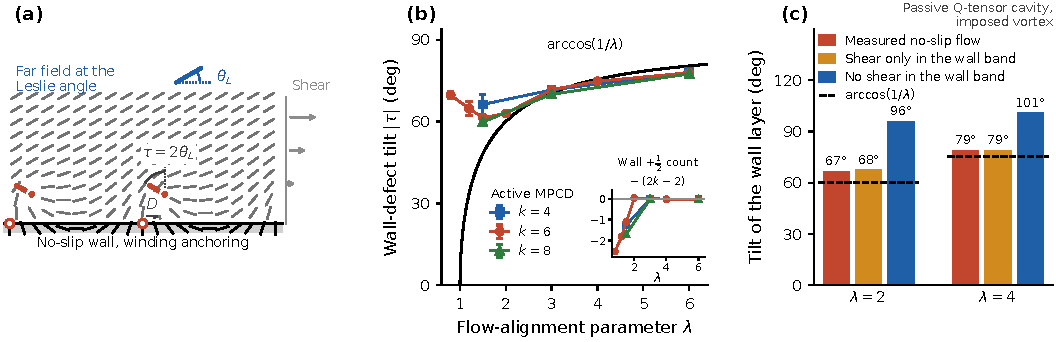
\includegraphics[width=\textwidth]{fig3_tiltlaw}
\caption{Origin of the tilt. (a) Flat no-slip wall with winding anchoring (one-constant solution): sliding the screening $+\half$ by $D$ from a homeotropic site
rotates the far field by $\kappa D$ and the defect by $2\kappa D$; in shear the far field settles at the Leslie angle $\theta_L$, so $\tau=2\theta_L=\arccos(1/\lambda)$.
(b) Wall-defect tilt in active MPCD circles (mean $\pm$ s.e.\ over seeds); inset: wall count minus $2k-2$. (c) Passive Q-tensor cavity under an imposed vortex:
tilt for three flow profiles.}\label{fig:tilt}
\end{figure*}

\paragraph*{The tilt angle.} Elasticity alone would tilt the layer by only $\approx35^\circ$. The angle comes from flow alignment in the shear next to the no-slip
wall. Consider a flat wall in simple shear with the anchoring winding along it. Translating the screening defect by $D$ rotates the far-field director by $\kappa D$
and the defect by $2\kappa D$ at no energy cost, which is Eq.~\eqref{eq:lock} as a zero mode. Far from the wall the director must sit at the Leslie angle
$\theta_L$ of the shear, $\cos2\theta_L=1/\lambda$. If the layer passes on no torque it slides along its zero mode until the far field is aligned, so
\begin{equation}
\tau=2\theta_L=\arccos(1/\lambda),\label{eq:tilt}
\end{equation}
independent of the shear rate and the elastic constants; only the ratio of strain to vorticity, fixed by the no-slip wall, enters. Flat-wall continuum simulations
confirm each step. Removing the shear next to the wall in the cavity model changes the tilt by 29$^\circ$ at $\lambda=2$ and 22$^\circ$ at $\lambda=4$, while confining all shear to the wall band leaves it
unchanged. In active MPCD circles the tilt follows Eq.~\eqref{eq:tilt} within $3^\circ$ for $\lambda=2$--6 (63.0, 71.7, 74.8, 77.9$^\circ$ against 60.0, 70.5, 75.5,
80.4$^\circ$) at $k=4$, 6 and 8 (Fig.~\ref{fig:tilt}). Below $\lambda\approx2$ the overcharged state itself breaks down. \todo{size dependence of the threshold from
runs/lamsize (batch 2, running 2026-10-14): coherence loss vs jet route}

% --------------------------------------------------------------------------------------------
%% FIG. 4 (beyond circles): (a) phase diagram: tilt coherence and vacancies vs aspect (phase_shapes c,a); (b) escape mechanism: wall-blocked jet g(d) and the untilting
%% run-up (jetmap c + etsg a, or a sketch); (c) wall law: bulk charge per unit length vs aspect, coloured by q, with the channel point (fig_perlength a or c);
%% SHIELDING (user, 2026-10-14; Japan-poster construction): potential of one bulk +1/2 from the layer alone, circle (3D surface, flat floor) vs aspect-2 ellipse
%%     with the measured depleted layer (wells at vacancies) -> panel (a') or a separate Fig. 4 row; source bulkdyn/fig_shielding_layer (a, c, f).
%% (d) MIRROR CONTROL: vacancies (or released charge) vs aspect for +k (wall +1/2, self-propelled) and -k (wall -1/2, not self-propelled), same cavities
%%     (TODO: server mirror shape sweep, 675 runs, after the circle seeds; preliminary: -1/2 layers hold, 1 size, 2 seeds).
\begin{figure*}[t]
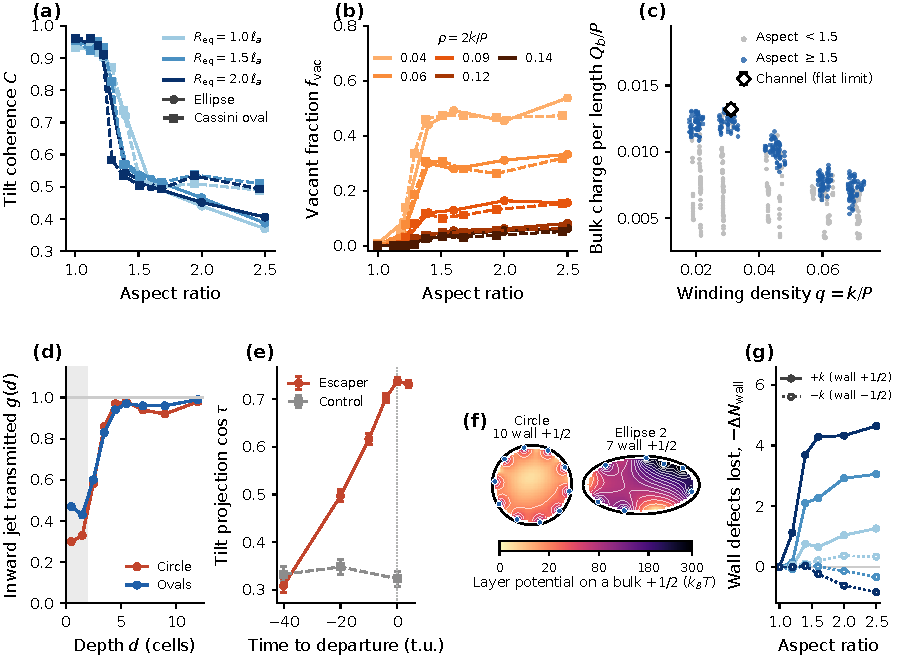
\includegraphics[width=\textwidth]{fig4_shapes}
\caption{Beyond circles. (a) Tilt coherence and (b) vacancies of the wall layer against aspect ratio for ellipses (solid) and Cassini ovals (dashed) at three
sizes. (c) Bulk charge per unit wall length against winding density $q=k/P$; elongated cavities (blue) collapse on a wall law, and the periodic channel (diamond)
is its flat limit. (d) Fraction of a wall $+\half$'s inward jet transmitted near the no-slip wall. (e) Escaping defects untilt over $\approx40$\,t.u.\ before
leaving; residents do not. (f) Potential of a bulk $+\half$ from measured layers: flat in the circle, tilted by $\approx180\,\kT$ in the depleted ellipse.
(g) Mirror control \todo{pending}.}\label{fig:shapes}
\end{figure*}

\paragraph*{Beyond circles: the layer leaks.} Elongating the cavity breaks the single coherent vortex at aspect ratio 1.25--1.37 for ellipses and ovals alike,
at every size; the active continuum model shows the same transition. The wall layer then loses defects one at a time. Following single escapes shows why the
tilt matters: each wall $+\half$ is self-propelled along its head, but the tilt turns its jet along the wall, and the no-slip wall transmits only $\approx30\%$
of the inward component within two cells (the wall-side vortex lobe of the defect is erased). An escaping defect first untilts over $\approx40$\,t.u., its jet
turns inward, and it runs away against an intact elastic barrier. \todo{one sentence on the steady state: unique dynamical balance, limited by layer crowding}

In a circle the evenly spaced layer shields the bulk completely: with same-sign wall images, the potential a bulk $+\half$ feels from the layer is flat
inside the ring apart from a corrugation next to it (a two-dimensional shell theorem; leftover range 1.6\,$\kT$ in the inner 60\%, Fig.~\ref{fig:shapes}(f)).
Elongation alone weakens this only to $\approx14\,\kT$, and fewer but evenly spaced wall defects only to $\approx27\,\kT$. The measured layers of aspect-2
ellipses are both depleted and unevenly spaced, and they do not shield at all: the potential tilts across the whole interior by $\approx180\,\kT$ (median), downhill
towards the largest gaps. \todo{trim; decide main text vs SM; the other bulk charges, absent here, partly screen this field}

In the circle the same construction explains the wall exchange. A full, count-locked layer leaves 17\,$\kT$ of field in the inner 60\%; a single vacancy or an
extra wall defect is an unscreened half-charge whose logarithmic field ($\approx140\,\kT$) spans the cavity, and with a vacancy it points at the hole in every
measured frame (Fig.~\ref{fig:vac}). Accordingly, an entry into the layer triggers an exit about five times sooner than chance (22 vs 104\,t.u.), usually of
another defect anywhere on the ring. \todo{CHECK with Benjamin before using: the maps show no potential drop near some layer defects and an asymmetry in the circle; tips of ellipses look unusually well shielded (see RESEARCH.md 2026-10-14 'TO REVIEW')}
\begin{figure}[t]
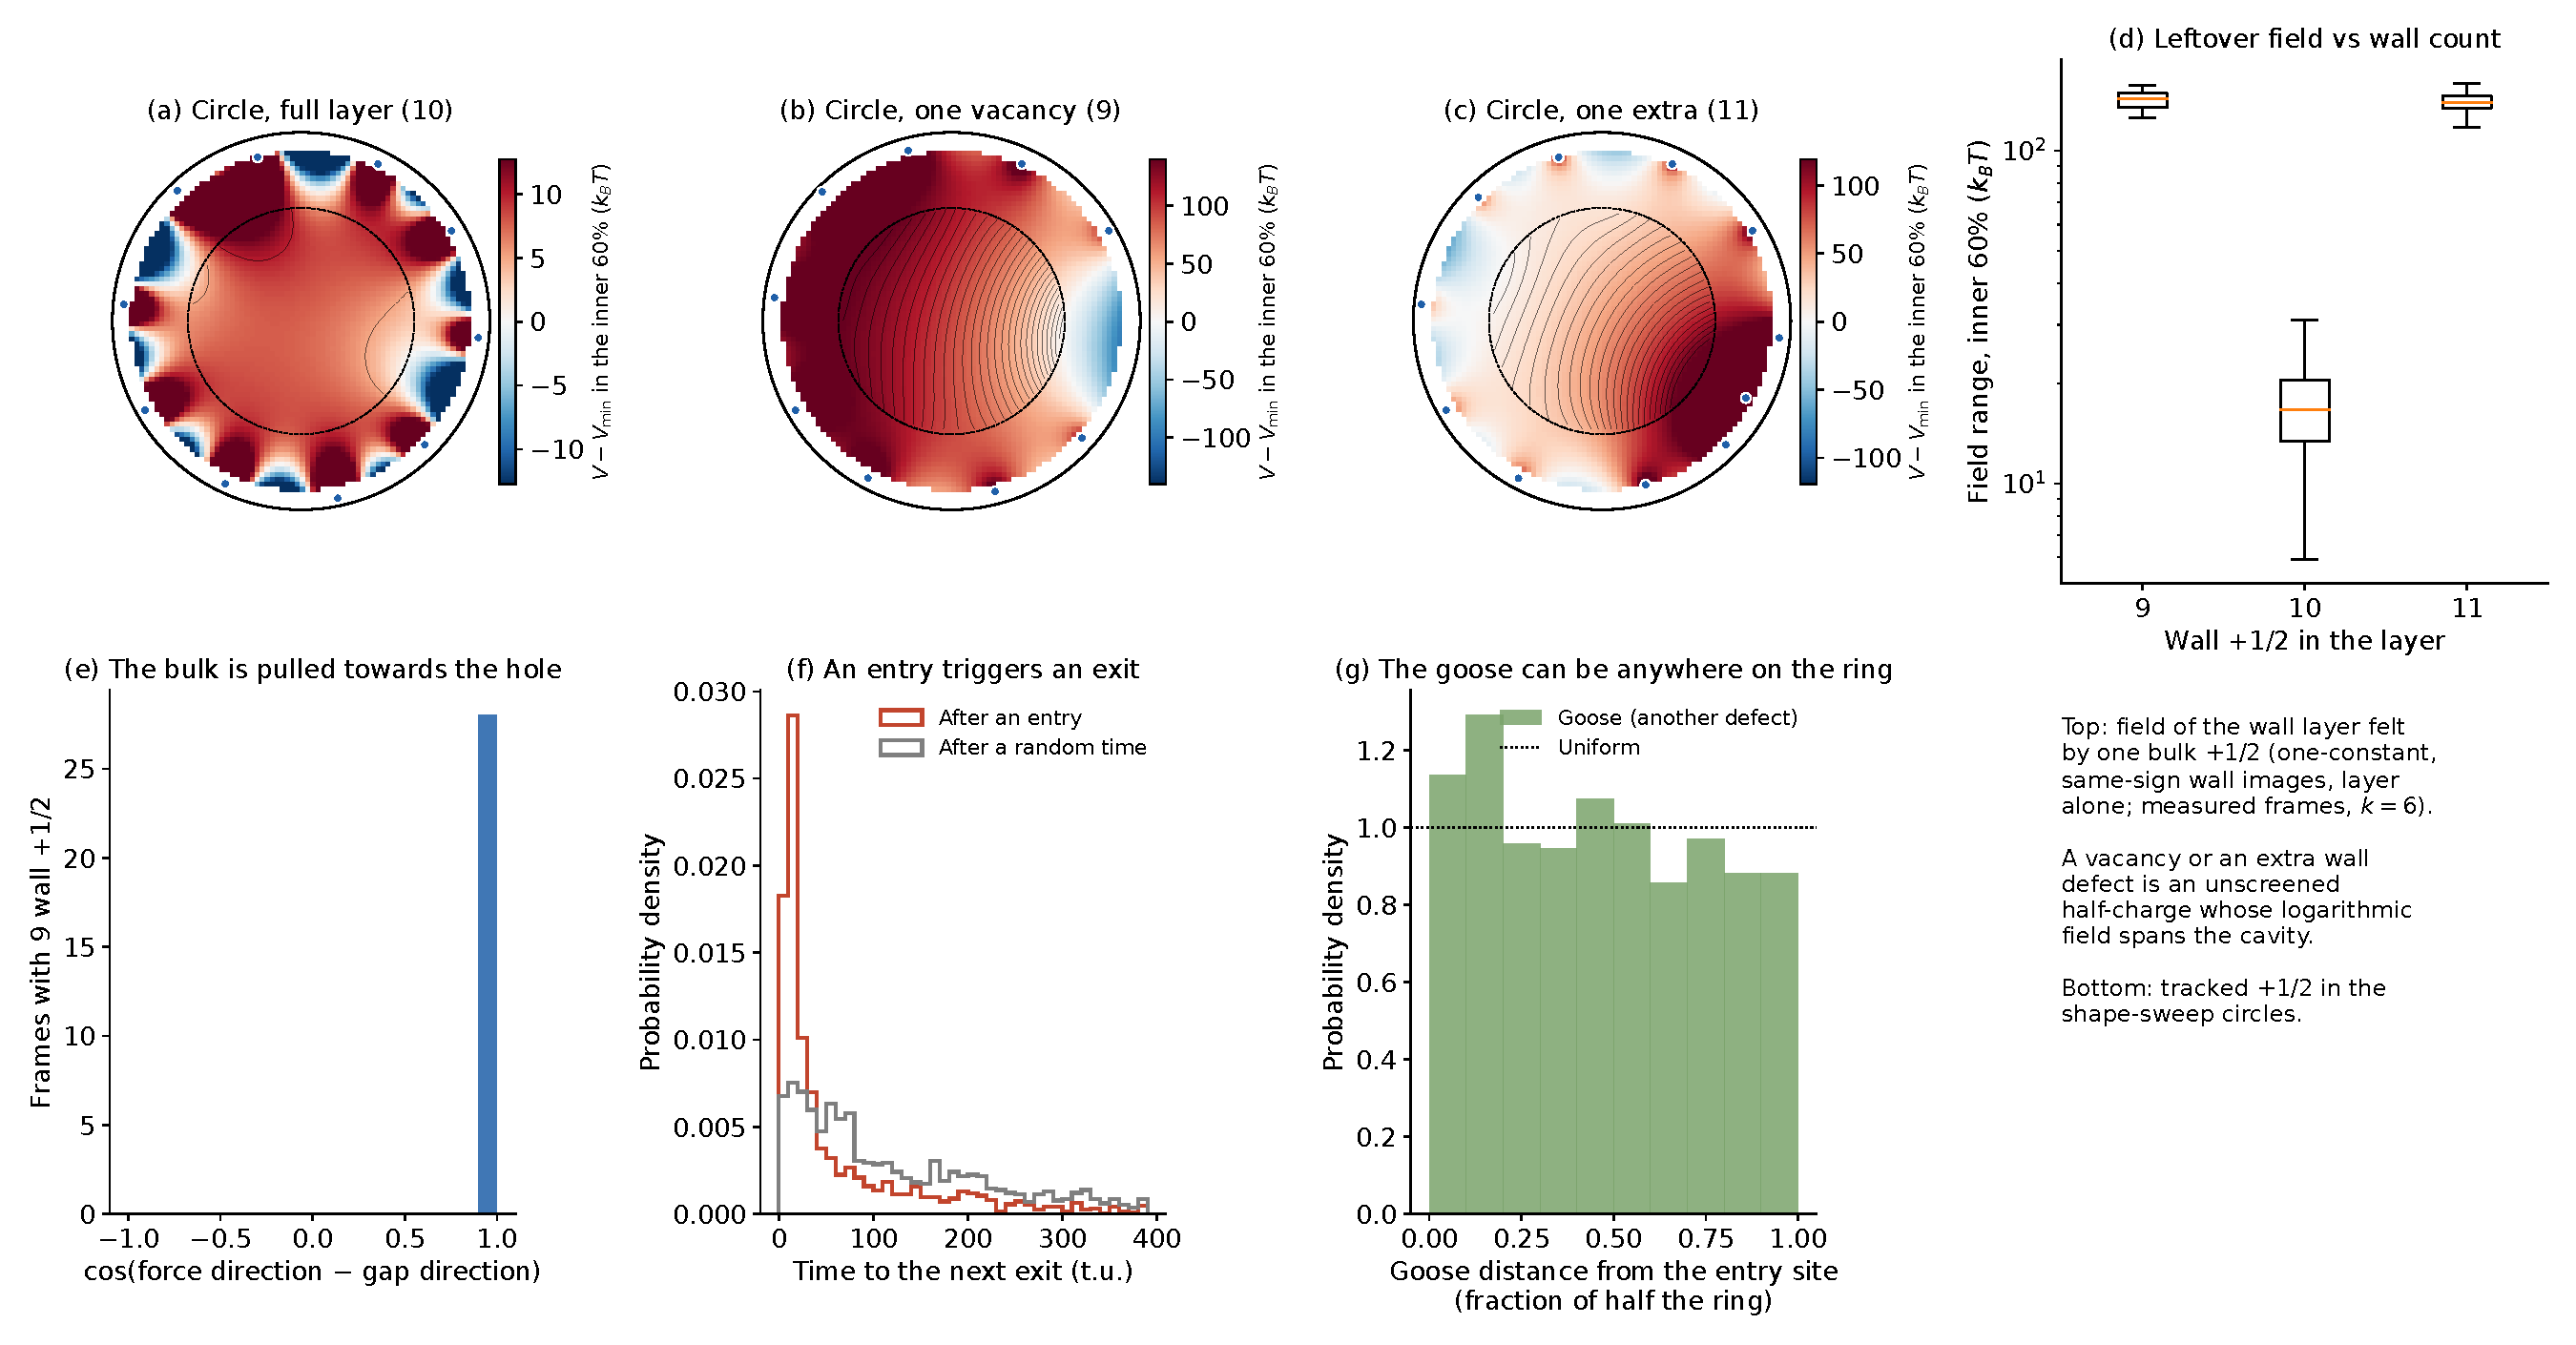
\includegraphics[width=\columnwidth]{fig_vacancy_field}
\caption{\todo{merge into Fig.~4 or SM}. Vacancy versus full layer in active circles ($k=6$). (a--c) Field of the layer felt by one bulk $+\half$ for a full layer, one
vacancy and one extra wall defect; (d) its range in the inner 60\% against the wall count; (e) with a vacancy the force on a bulk $+\half$ points at the hole;
(f) time to the next exit after an entry into the layer vs after a random time; (g) position of the defect that leaves (`goose') relative to the entry site.}\label{fig:vac}
\end{figure}

The released charge obeys a wall law (Fig.~\ref{fig:shapes}). Above aspect $\approx1.5$ the bulk charge per unit wall length no longer depends on shape or size
and is set by the winding density $q=k/P$ alone, $Q_b\approx c(q)P$, with $c\approx0.012$ at $q\approx0.03$; denser windings release a smaller fraction
(0.61 at $q=0.02$, 0.11 at $q=0.07$). A periodic channel with the same winding density, the flat limit of the cavities, releases the same share. Circles are the
exception: they hold exactly $+1$ at every size, the topologically protected case.

\paragraph*{Mirror control.} \todo{MIRROR SHAPE SWEEP (server, pending). Reversing the winding ($k\to-k$) makes the wall layer of $-\half$ defects, which are not
self-propelled. If the leak is driven by the wall defects' own jets, $-\half$ layers in the same elongated cavities should hold. Preliminary (one size, two seeds):
they hold, with a stronger restoring force. Also state the circle result: the $-\half$ layer gains about 1.5 of the 2 defects predicted by the continuum
(13--13.5 of 14, unique from seeded starts), so MPCD and continuum differ for negative winding (open). One sentence + Fig.~\ref{fig:shapes}(g) + SM Sec.~S12.}

% --------------------------------------------------------------------------------------------
\paragraph*{Discussion.} \todo{(1) what is general: any flow-aligning active nematic with patterned anchoring; the law has no free parameter. (2) Experimental
proposal: microtubule/kinesin or cell monolayers in wells with patterned winding anchoring; predicted tilt and charge. (3) Open: negative winding (MPCD gains
1.5 of the 2 predicted $-\half$), onset $R/\la$ and its $k$-ordering.}

\begin{acknowledgments}
\todo{acknowledgments, funding, computing}
\end{acknowledgments}

\bibliography{../refs}

\end{document}
